\documentclass[conference]{IEEEtran}
\IEEEoverridecommandlockouts

% to be able to draw some self-contained figs
\usepackage{tikz}
\usepackage{amsmath}

\usepackage{listings}
\usepackage{parcolumns}
\usepackage{graphicx}
\usepackage{caption}
\usepackage{subcaption}
\usepackage[inline]{enumitem}


\usepackage{hyperref}

\renewcommand\sectionautorefname{Section}  
\renewcommand\subsectionautorefname{Section}
\renewcommand\subsubsectionautorefname{Section}
\renewcommand\itemautorefname{Attack}
\renewcommand\figureautorefname{Figure}
\renewcommand\tableautorefname{Table}

% Comment macros
\newcommand{\uros}[1]{\textcolor{pink}{\textbf{UT:} #1}}
\newcommand{\pra}[1]{\textcolor{blue}{\textbf{PS:} #1}}
\newcommand{\nb}[1]{\textcolor{green}{\textbf{NB}: #1}}
\newcommand{\mat}[1]{\textcolor{red}{\textbf{Mat:} #1}}
\newcommand{\evalfull}[1]{20}
\newcommand{\evalnocalls}[1]{3}
\newcommand{\sysname}{TikTok}
\newcommand{\roughevaloverheadbad}{17\%}
\newcommand{\roughevaloverheadbetter}{2-6\%}



%-------------------------------------------------------------------------------
\begin{document}
%-------------------------------------------------------------------------------

%do not want date printed
\date{}

% make title bold and 14 pt font (Latex default is non-bold, 16 pt)
\title{\Large \bf TikTok: Kernel TOCTTOU Protection}

%for single author (just remove % characters)
\author{
Anonymous submission \#303 to Security \& Privacy '21
%{\rm Eric Tusso}\\
%EPFL
%\and
%{\rm Yamaha Priest}\\
%EPFL
% copy the following lines to add more authors
% \and
% {\rm Name}\\
%Name Institution
} % end author

\maketitle

%-------------------------------------------------------------------------------
\begin{abstract}
%-------------------------------------------------------------------------------

Double-fetch bugs are a plague in all major operating system kernels.  They
occur when data is fetched twice across the trust-boundary without checking that
it has not changed. Such bugs may force the kernel into an inconsistent state,
allowing an attacker to illegally access memory, cause denial of service, or to
escalate their privileges.

So far, the only protection against double-fetch bugs is to detect and fix them.
However, they exhibit illegal behavior only under specific conditions, making
them incredibly hard to find. Even worse, the bug may be in unchangeable code
(e.g., a binary driver blob).
%
We propose \sysname{} to mitigate double-fetch bugs.  \sysname{} leverages
on-the-fly page-table hardening to prevent changes to the system call arguments,
while the system call executes.


\sysname{} shows no noticeable drop in performance when evaluated on CPU-bound
workloads. On extremely system call heavy workloads, \sysname{} shows
\roughevaloverheadbetter{} overhead when protecting select system calls, and
\roughevaloverheadbad{} when all system calls are guarded.


\end{abstract}

\begin{IEEEkeywords}
Double-fetch bugs, TOCTTOU, kernel security, page-tables, mitigation
\end{IEEEkeywords}

% Talk about the system call filters and how they can be used for good
% Introduce the main problem - TOCTTOU
% Brag how our system is the best thing since sliced bread
\section{Introduction}

% Syscalls are a lucrative attack surface for adversaries which needs to be protected
Modern systems consist of \emph{untrusted} user-space processes and the
\emph{trusted} kernel.  All data that crosses this trust boundary must be
checked.  Double-fetch bugs~\cite{serna08doublefetch, twizsgrakky07ring0,
wilhelm2016xenpwn, wang2018survey} occur when higher-privileged code (e.g., the
kernel) reads the same data twice from a lower-privileged address space (e.g.,
user-space). As attackers may change the data between the two reads, this
enables a plethora of attack vectors.  Double-fetch bugs are a type of
\emph{race condition} between threads of different privileges. A
\emph{Time-of-check to time-of-use (TOCTTOU)} violation occurs when the first
read is used to check the operand while the second read is used to modify
state.  Double-fetch bugs are a frequent problem in kernels and
hypervisors~\cite{cve201812633, cve202012652, cve20131332, cve201920610,
cve20158550, cve201610439, cve201610435, cve201610433, cve20195519,
cve20168438}. Considering that double-fetches also appear in drivers, legacy
systems with binary-only drivers cannot be patched, even if a bug is found.
Furthermore, Watson~\cite{watson2007exploiting} blames an unfixable TOCTTOU bug
as a reason for the insecurity of \emph{system call wrappers}.  

% Enumerate the attack vectors
This state of affairs calls for a solution that \emph{mitigates} double-fetches in
system calls to protect the kernel.
To mitigate double-fetch bugs, a system must prohibit changes from
concurrent threads to memory accessed by the system call.
The comprehensive system that protects against the modification of arguments
must consider all possible approaches to change the arguments.
Possible attack vectors are:
\begin{enumerate*}[label=\textbf{(\roman*)}]
\item  direct writes from user-space,
\item  kernel writes from system calls,
\item  remapping the pages with different permissions,
\item \texttt{write} calls to a file that alter mapped
file pages, or
\item  storing arguments on device-backed pages
\end{enumerate*}.
Simply preventing direct writes from user-space is insufficient to stop these attacks.
A mitigation must monitor redundant mappings, system calls, and write
calls to files.

% Explain how we protect against the attacks briefly
% \emph{Marking} pages \emph{read-only} when system call arguments are read
% the first time prevents \autoref{attk:direct} and \autoref{attk:systemcall}. As
% the page is loaded into the memory space, it is checked if it is already marked.
% The permissions of the mapping are adjusted if necessary. This defends against
% \autoref{attk:remapping}. Pausing system calls that write to a file while some
% of its mapped pages are marked prevents \autoref{attk:writebuffers}. Finally,
% \autoref{attk:devicefiles} can be prevented by stopping the adversary from
% mapping devices through \emph{Discretionary Access Control (DAC)}.

% Simplified mitigation description
Our proposed mitigation \emph{marks} user-space pages touched by kernel code as
\emph{read-only} to prohibit the first two attacks (direct writes from concurrent
user-space threads or concurrent system calls). Whenever a page is linked into
an address space, its security properties are checked to mitigate the
third attack (remapping). If a file is mapped to memory then write system calls
are paused if the target page is marked to mitigate the fourth attack (write
buffers). We prevent the fifth attack through
through \emph{Discretionary Access Control (DAC)} for device-backed pages.
%
% A really high level overview of how the system works
Our mitigation relies on a well-defined interface for \emph{reading} (\texttt{read\_in})
from user-space and on the paging infrastructure to protect marked pages.
Threads that write to a marked page are paused in the
\emph{page-fault handler} and continue after the page is
unmarked. The kernel interface for \emph{writing} (\texttt{write\_out}) to
user-space is extended to execute all writes to marked pages at the end of the
call. This prevents the system calls from writing to the pages they have marked.
%
A small set of system calls (e.g., \texttt{pollfd}, \texttt{futex}, or
\texttt{sys\_nanosleep}) depend on ``double-fetch-like'' behavior and need to be
manually verified and whitelisted.

% % Overview of the limitations
% A small subset of system calls (e.g. \texttt{pollfd}, \texttt{futex}) depends on
% the writes from user-space or double-fetches for the correct behavior.
% Similarly, certain system calls take a long time to execute
% (\texttt{sys\_nanosleep}). They keep their arguments marked for the duration of
% the call, hurting performance. These groups of system calls should have the
% protection disabled and be manually inspected (or better formally verified) to
% ensure absence of double-fetch bugs.

% Introduce TikTok
We implement our mitigation, \sysname{}, as a memory marking extension to the
Linux kernel that does not require any changes to user programs.
\sysname{} provides system calls with a memory snapshot of when
pages have first been read during that system call.
\sysname{} groups all writes that modify protected memory and batches them at
the end of the system call. By mitigating
double-fetches, \sysname{} protects against the double-fetch bugs in all kernel
code. Furthermore, \sysname{} renders
previously unavoidable double-fetches (such as a TOCTTOU in system call
wrappers) completely benign. 
% \sysname{} works on modern Linux distributions
% (Ubuntu Server 18.04 LTS) and does not require any modifications to the user
% programs. It can be implemented in other kernels and architectures which use
% page-tables and a well-defined API to communicate with the user space
% (\texttt{read\_in} and \texttt{write\_out} abstractions).

% Sneak-peek into the results

Our evaluation shows that extremely system call heavy multithreaded programs,
such as Apache and NginX, suffer an \roughevaloverheadbad{} drop in performance
with \sysname{} protecting all possible system calls. Whitelisting high
frequency system calls drops the overhead to \roughevaloverheadbetter{}. CPU-bound
programs show negligible performance loss, even when they
use multiple threads (OMP~\cite{dagum1998openmp}) or multi-process
message-passing (MPI~\cite{snir1998mpi}).



% Four contributions
The main contributions of this paper are:

\begin{itemize}

% Atri's comment: Why is the attack a separate contribution? Ans: It is an interesting attack vector
\item A \emph{confused deputy attack} on memory-marking protection mechanisms
that mark the pages with a \emph{superuser} bit, % (\autoref{attk:systemcall})
\item A solution to the problem of protecting the arguments of system calls that
write to their arguments,
\item A comprehensive technique for temporarily preventing memory from being
      changed, by safely postponing updates from both user-space and kernel, and
\item \sysname{}, a mitigation for the double-fetch and TOCTTOU attacks on
      system call arguments in the Linux kernel.
\end{itemize}

% Cover the theory needed to understand how and why TikTok works
% 1) IPC - We need this to argue why the deadlocks are almost impossible
% 2) VM and Page Tables - Why it exists and how it works
% 3) x86 Page Tables - Continue the discussion from the previous section
% 4) Page faults - Explain how and why they happen.
% 5) Copy to/from user - Explain why the API has been introduced
% 6) Double-fetches - Provide a high-level overview
\section{Background}
\label{sec:background}

\sysname{} orchestrates several Linux subsystems to provide its protection. It
uses \emph{page-tables} to mark \emph{shared memory} storing the system call
arguments as \emph{read-only}. Different system calls have different
relationships with shared memory, and interact with \sysname{} differently in
practice. This section provides the background information necessary to reason
why and how \sysname{} protects the arguments from change while enabling the
threads to execute correctly.

% I want to cover why this background is needed. IPC is the most problematic
% because it is used to justify the absence of deadlocks
\autoref{subsec:ipc} introduces two different ways of communication between
processes - \emph{shared memory} and \emph{message-passing}. \sysname{} affects
both of these methods because the arguments of the message-passing system calls
are stored in (potentially shared) memory. The waits caused by writing to marked
pages can interact with already present synchronization primitives and cause
deadlocks. In~\autoref{subsec:deadlocks} we explain why they do not appear in
practice.

\autoref{subsec:vm} covers the organization of \emph{virtual memory},
\emph{page-tables} and the interface the Linux kernel uses to access the
user-space memory. This section is essential to understanding the implementation
of \sysname.

\autoref{subsec:doublefetch} details the \emph{double-fetch} bug that \sysname{}
is mitigating. It explains its cause and the different types of double-fetch bugs.


\subsection{Interprocess Communication}
\label{subsec:ipc}

The two methods of inter-process communication are  \emph{shared memory} 
and \emph{message passing}~\cite{silberschatz2018operating}.

% Intro to shared-memory
% Intro to message-passing
Shared memory relies on two processes having a section of memory that both can 
access. Processes communicate by reading and writing to the shared memory.
Message passing consists of one process calling \texttt{send}, and another one
calling \texttt{receive} to fetch the message. Synchronous message passing
blocks execution until the calls have finished.

% The state of the modern OSs and concurrent programs
Modern operating systems support both of these approaches. \sysname{} interferes
with message-passing system calls by linking them to shared memory. Storing
arguments for blocking message-passing system calls in shared memory can cause
deadlocks if those arguments are written to (see~\autoref{subsec:deadlocks}).

\subsection{Linux Memory Subsystem}
\label{subsec:vm}

% Paged VM and the introduction to permissions we will later use in TikTok
Linux implements \emph{paged virtual memory} and uses \emph{virtual addresses}
which map to \emph{physical addresses} in RAM. The mapping function is defined
for each process by a multi-level \emph{page-table}.

% The flags are needed to discuss marking
The leaves of the page-table store the access information about the
corresponding page:
\begin{LaTeXdescription}
    \item[Present bit (\textbf{P})] is set if the page is present in memory
    \item[Read/Write bit (\textbf{R/W})] denotes if the page is writable or just
         readable
    \item[User/Superuser bit (\textbf{U/S})] represents if the page can be 
    accessed by the user, or only by the superuser
    \item[Not Executable bit (\textbf{NX})] is set if the code stored on the 
    page cannot be executed
    \item[Page Frame Number] denotes the page frame the entry points to
    \item[\textbf{SW1-SW4}] Four bits free for the OS to use
\end{LaTeXdescription}

% Mention TLBs
Considering that the page-table traversal is frequent, it is implemented in
hardware by the \emph{memory management unit} (MMU). Reading the page-table from
memory is slow, so a small cache---\emph{translation-lookaside buffer} (TLB)
--- is added to the MMU to store frequently accessed page entries. Kernel
developers can \emph{flush} (clear) certain TLB ranges in software.

% Explain what a page fault is, as well as COW (mentioned later as an optimization)
On invalid access (e.g., wrong permissions, page not present) the MMU will
trigger a page-fault. The page-fault handler executes in the kernel context of
the faulting thread and performs the appropriate action (e.g. load a page, kill
the thread). With the advent of cloud computing, \emph{user-space page-fault
handling} has been added to the Linux kernel. \sysname{} relies on the page-fault
handler for protection, so user-space page-fault handling must be disabled.

% Different memory types used later to explain certain attacks
Memory in Linux can be either \emph{file-backed} or \emph{anonymous}.
File-backed pages have a backing file where their data is stored. Anonymous
pages do not have a backing file (e.g., stack and heap) and the data on them
disappear when they are unmapped.

Another classification is based on privacy: \emph{private} and \emph{shared}.
Private memory is part of only one virtual memory space. This memory space can
be accessed by multiple threads in a process, but not by other processes. Shared
memory can be accessed by different processes.

% This is the most important paragraph and a basis for one of the attacks. The
% previous two paragraphs are just the introduction
Shared file-backed pages are of interest because their content does not
disappear when they are unmapped, and they can be mapped by multiple
processes at different times. This makes them suitable for mounting elaborate
attacks on memory-marking systems.

\subsection{Copy-from-User and Copy-to-User}
\label{subsec:copy}
% The interface for communicating with the user-space and why it exists
Linux differentiates between accesses to user-space and kernel memory and
therefore uses a well-defined interface when accessing user-space memory.
User-space memory can be written to the disk and evicted from the main memory.
Accessing absent pages triggers a page-fault handler, where they are read back
to memory. Kernel memory pages are always present and triggering a page-fault
handler in the kernel is considered a serious error. The kernel uses a well-defined
interface that handles possible page-faults when accessing user-space:
\texttt{(\_\_)copy\_(from/to)\_user}, \texttt{(\_\_)(get/put)\_user},
\texttt{user\_str(cpy/len)}. When the actual implementation is not important,
this API is refered to \texttt{read\_in} and \texttt{write\_out}. \sysname{}
extends this interface to perform additional checks and the bookkeeping of
marked pages.

\subsection{Double Fetch Bugs}
\label{subsec:doublefetch}

\begin{figure}[]
  \centering
  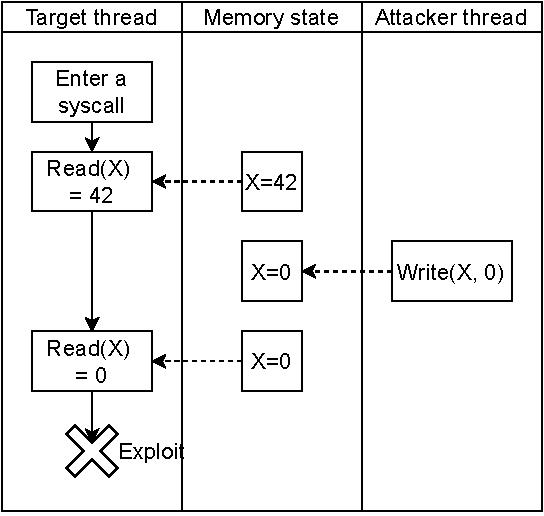
\includegraphics[width=.85\linewidth]{img/doublefetch.pdf}
  \caption{Diagram of a double-fetch bug.}
  \label{fig:doublefetch}
\end{figure}

\begin{minipage}{\linewidth}
  

\begin{lstlisting}[language=C, caption={Abridged CVE-2018-12633 Double Fetch.},
                  label=code:cvedoublefetch,  breaklines=true, captionpos=b,
                  postbreak=\mbox{\textcolor{red}{$\hookrightarrow$}\space},
                  numbers=left,basicstyle=\scriptsize, xleftmargin=5.0ex]
static long vbg_misc_device_ioctl(
        struct file *filp,
        unsigned int req,
        unsigned long arg)
{
  size_t size;
  struct vbg_ioctl_hdr hdr;
  void *buf;

  if (copy_from_user(&hdr, (void *)arg, sizeof(hdr))) 
    return -EFAULT;
  
  if (hdr.version != VBG_IOCTL_HDR_VERSION) 
    return -EINVAL;
   
  if (hdr.size_in < sizeof(hdr) || (hdr.size_out && hdr.size_out < sizeof(hdr)))
    return -EINVAL;
  
  ...
  
  if (copy_from_user(buf, (void *)arg, hdr.size_in)) {
		ret = -EFAULT;
		goto out;
  }

  ...

  ret = vbg_core_ioctl(session, req, buf);

  ...
}
\end{lstlisting}
\end{minipage}
% The idea behind double-fetch bugs
\emph{Double-fetch} bugs occur when a privileged environment (such as the
kernel) reads untrusted memory two or more times and the read values are not
identical (\autoref{fig:doublefetch}). In between those two reads, memory could
have been changed by an unprivileged adversary. Considering that the bug relies
on carefully timed accesses for two different threads, it is a race
condition. The situation where the first fetch validates the value of the
fetched variable, but the computation is only performed on the second fetch, is
called a \emph{time-of-check to time-of-use} (TOCTTOU) bug. TOCTTOU bugs have
been widely studied in file systems, where the API makes it possible to swap the
file after validating the access rights~\cite{payer2012protecting,
pu2006methodical, wei2010modeling, tsafrir2008portably}.

% Explain using the example
\autoref{code:cvedoublefetch} displays the double-fetch bug in the Virtual Box
drivers for the Linux kernel~\cite{cve201812633}. The first fetch occurs on line
10. The code gets the header, checks the arguments (lines 13 -- 17)
and fetches the whole argument into the variable \texttt{buf} (line 21). The new
value is then used (line 27).

% The bug and the fix
Note that the header is fetched twice---on lines 10 and 21. This gives the
opportunity for the attacker to change the values. Considering
that the header is not verified the second time, the attacker can
leave the kernel in an inconsistent state. The fix for this bug
(\autoref{code:cvedoublefetchfix}) does not fetch the header the second time. It
copies the header into \texttt{buf} and the second fetch skips it.

\begin{lstlisting}[language=C, caption=CVE-2018-12633 Double Fetch Fix~\cite{cve201812633fix},
  label=code:cvedoublefetchfix,  breaklines=true, captionpos=b,
  postbreak=\mbox{\textcolor{red}{$\hookrightarrow$}\space},
  numbers=left,basicstyle=\scriptsize, firstnumber=18, xleftmargin=5.0ex]
...

  *((struct vbg_ioctl_hdr *)buf) = hdr;
  if (copy_from_user(buf + sizeof(hdr), (void *)arg + sizeof(hdr), hdr.size_in - sizeof(hdr))) {
    ret = -EFAULT;
    goto out;
  }

...

\end{lstlisting}

% Double-fetches are actually so big that people have actualy spent time
% to study them
Wang et al. explain in~\cite{wang2018survey} that double-fetches appear not only
in kernels, but wherever there is a trust boundary to cross (e.g., kernel ---
hypervisor~\cite{wilhelm2016xenpwn} and hardware---kernel
boundaries~\cite{lu2018untrusted}). Double-fetches have been responsible for many
vulnerabilities in different kernels~\cite{jurczyk2013bochspwn, wang2018survey}.


\section{Threats and Attacks}

We now describe the threat model and attacker capabilities along with the
attacks that can be mounted to change the data in memory, to exploit a
double-fetch bug.


\subsection{Threat Model}
\label{sec:threatmodel}

% Nothing fancy -- the adversary is just trying to hack the system
% No black magic allowed
The adversary has access to a user account on the target machine. They can
execute arbitrary code, including system calls. Some of the system calls
have double-fetch vulnerabilities, and the adversary wants to exploit them,
e.g., for privilege escalation.

The attacker may execute an arbitrary sequence of system calls. \sysname{}
mitigates any unintended corruption or information leakage \emph{in the kernel}
or \emph{in other user processes} that arises through
double-fetch bugs. Hardware attacks such as Rowhammer~\cite{mutlu2019rowhammer}
or side-channels~\cite{kocher2019spectre}, and file-system TOCTTOU
attacks~\cite{payer2012protecting, pu2006methodical, wei2010modeling,
tsafrir2008portably} are out of scope.

\subsection{Attacks Classification}
\label{sec:attacks}

% List five attacks and explain them quickly
\sysname{} guards data passed into the kernel against different forms of
modification. While writes from user-space and the kernel are straight forward,
there are also subtle ways to evade the protection of a memory-marking system. 
A non-obvious attack vector focuses on memory remapping, e.g., concurrent calls
to \texttt{mmap}, remapping the same region multiple times, or writing to an
opened but mmapped file.
Most of these attacks could be prohibited by disabling file-mappings but this
would negatively impact software compatibility.
Linux relies on multiple page mappings and file mappings to provide shared-libraries and load
programs into memory.
The following attacks are possible:
\begin{enumerate}
  \item \label{attk:direct} \emph{Direct double fetch} consist of a malicious
  user trying to directly write to the argument stored in memory, while the
  system call is executed in another thread. 

  \item \label{attk:systemcall} \emph{Privileged double fetch} are indirectly triggered.
  The user performs a \texttt{read} system call with the target address as the
  destination. The data is then written to this location by the \texttt{read}
  system call from the kernel.

  \item \label{attk:remapping} \emph{Reflected double fetch} is accomplished by
  mapping marked pages in another process. The malicious user stores the
  arguments on a file-backed page and maps the file again as writable, while the
  system call is executing. The user is then free to write to the new mapping,
  even though \emph{other mappings} are read-only. 

  \item \label{attk:writebuffers} \emph{Inception double fetch}
  bypasses the protections present in user-space mappings by directly changing
  the data present in the files.

  \item \label{attk:devicefiles} \emph{Device double fetch} can change
  independently of writes. Storing arguments on such pages can result in reading
  different values from them, even if no writes occur in-between the reads.

\end{enumerate}

Watson~\cite{watson2007exploiting} in his analysis of CerbNG introduces
\autoref{attk:direct}, \autoref{attk:remapping} and \autoref{attk:writebuffers}.
We extend the discussion of known attacks and introduce
\autoref{attk:systemcall} and \autoref{attk:devicefiles}.


%%%%%%%%%%%%%%%%%%%%%%%%%%%
\section{\sysname{} Design} \label{sec:design}
%%%%%%%%%%%%%%%%%%%%%%%%%%%

Designing a memory-marking system is prone to pitfalls. A naive design would
instrument \texttt{read\_in} to \emph{mark} the pages it accesses with a
\emph{superuser} flag in the page-table and force the writers to \emph{wait} in
the page-fault handler. When returning from the system call marked pages are
\emph{unmarked}, and waiting writers are woken-up. Marking the page in all VM
spaces renders it unwritable by all user processes. However, calling
\texttt{read} with the page as the destination will bypass such a system. System
calls execute with superuser privileges and are allowed to write to protected
pages.

Based on our study of memory marking systems, we introduce the following design
principles to mitigate double-fetches:

\begin{itemize}
  \item \label{policy:immutability} \emph{Temporary Immutability:} Pages storing
  system call arguments become immutable after being read;
  \item \label{policy:exactness} \emph{Exactness}: Writes to protected pages
  do not affect the execution of the threads performing them; and
  \item \label{policy:correctness} \emph{Correctness:} The only way to change the
  protected pages is by writing to them.
\end{itemize}

By enforcing these three principles, the system mitigates double-fetch bugs and
protected programs execute correctly.

The naive design violates several of our design principles. Data can still be
changed because it does not protect against arbitrary memory mapping. Users can
bypass the protection by mapping guarded pages as writable in another process
(\autoref{attk:remapping}). Self-writing calls do not execute correctly---they
deadlock when writing to their arguments. Watson~\cite{watson2007exploiting}
mentions self-writing calls as a fundamental problem for memory-marking systems.
Finally, the naive design prevents writes from updating the memory. Memory
locations that can change independently, such as memory mapped device registers,
invalidate the protection (\autoref{attk:devicefiles}).

\sysname{} marks guarded pages as \emph{read-only}. While read-only pages will
prohibit privileged code from writing to it, some system calls (e.g.,
\texttt{rt\_sigaction}) write to the arguments they read and will deadlock.
\sysname{} accommodates these special system calls following the introduced
design principles.



% Nobody can change the marked pages. We mark them when the arguments are read
% and when the pages are mapped
\subsection{Temporary Immutability} \label{subsec:tempimmut}
%%%%%%%%%%%%%%%%%%%%%%%%%%%%%%%%%%%

Temporary Immutability of argument pages guarantees that repeatedly reading from
the same location returns the same data.

\sysname{} relies on the
page-table and the page-fault handler to provide immutability. The interface for
reading from the user-space (\texttt{read\_in}) is extended to change the
permissions of the pages being read to \emph{read-only}. The pages need to be
marked in all VM spaces. Otherwise, the adversary could write to the
page from a different process.

\sysname{} extends the mapping of pages to make sure the guarded pages are marked in
all processes. This protection holds even if they are mapped as writable after
being marked by another process. If the OS supports \emph{on-demand paging} the
marking should happen when the page is accessed and loaded by the process.

Temporary immutability prevents \autoref{attk:direct}, \autoref{attk:systemcall}
and \autoref{attk:remapping}.


% This is the most problematic section. Programs need to execute correctly.
\subsection{Exactness} \label{subsec:exactness}
%%%%%%%%%%%%%%%%%%%%%%

Self-writing system calls are problematic for memory-marking systems. Some
system calls rely on double-fetches and user-space writes to the arguments to
execute correctly. \sysname{} also introduces additional synchronization points
to user-space programs, requiring a deadlock prevention strategy. \sysname{}
preserves the equivalent execution of these system calls and user-space
programs. 

% The solution to the problem of a system call marking A and writing to it.
% Nobody has done this before.
\emph{Self-writing system calls} are addressed by preventing them from writing
to marked pages and triggering a page-fault. When a page is marked, it is also
added to a data structure containing marked memory memory ranges for each VM
space. We change the interface for writing to user-space (\texttt{write\_out})
to check if it is writing to a marked page. Our added data structure records the
writes to marked pages, and executes them at the end of the call, after
unmarking the arguments. This guarantees that system calls will not wait for
themselves to unmark the pages.  Watson~\cite{watson2007exploiting} stressed
that no system call wrappers had successfully addressed this problem.

% Some calls do not like TikTok. They want to read data multiple times. They are
% ignored
\emph{System calls that depend on double-fetches} cannot be protected by
\sysname{}, so they must be \emph{whitelisted} so that they do not mark
pages. \autoref{table:whitelist} provides a list of these system calls and a
reason why each system call needs whitelisting.. They
must be manually inspected for bugs. Whitelisting them does not diminish the protection
of other calls. Whitelisted calls still stop before writing to marked pages.

\begin{table}[]
  \begin{tabular}{|l|l|}
  \hline
  Whitelisted System Call & Reason                                 \\ \hline
  \texttt{futex}                   & Relies on outside writes               \\ \hline
  \texttt{poll}                    & Relies on outside writes               \\ \hline
  \texttt{ppoll}                   & Relies on outside writes               \\ \hline
  \texttt{select}                  & Relies on outside writes               \\ \hline
  \texttt{pselect6}                & Relies on outside writes               \\ \hline
  \texttt{rt\_sigtimedwait}        & Relies on outside writes               \\ \hline
  \texttt{execve}                  & Remaps memory                          \\ \hline
  \texttt{nanosleep}               & Keeps pages marked while it sleeps \\ \hline
  \end{tabular}
  \caption{Whitelisted system calls.}
  \label{table:whitelist}
  \end{table}

The best representatives are \texttt{pollfd}, \texttt{futex}, and
\texttt{execve}. \texttt{pollfd} checks if any of the file-descriptors in the
array passed as an argument are ready to perform I/O. The user can write
\texttt{-1} to memory to indicate that the loop in the call needs to skip the
descriptor. \texttt{futex} is a mostly user-space lock. Most of \texttt{futex}
synchronization depends on atomic user-space writes, with the system call being
performed only to awake or make threads wait. If \texttt{futex} marks a
user-space address as read-only, other user-space threads will be incapable of
unlocking the \texttt{futex} by writing to that address. \texttt{execve}
detaches the VM space and creates a new one. Whitelisting it
simplifies the detaching and destruction of VM spaces in \sysname{}.

Even though they execute correctly under \sysname{}, long-lasting calls (such as
\texttt{sys\_nanosleep}) should be included in this group. Otherwise, they could
keep the pages marked for long periods, sometimes preventing the program from
executing in reasonable time.

Finally---if a system call can be verified not to have double-fetches, it can
be whitelisted to improve performance. This is especially important in case of
system calls with large arguments such as \texttt{write}.

% The big problem. Deadlocks can occur if you are insane.
\subsection{Preventing Deadlocks}
\label{subsec:deadlocks}

% Introduce the problem
\sysname{} provides its guarantees by introducing additional synchronization
points to executing programs. It neither introduces deadlocks
by interacting with itself, nor
by interacting with blocking system calls.

% Explain why TikTok cannot cause a deadlock on its own
\sysname{} cannot cause a circular locking dependency as a consequence of its
\emph{system call reads, system call writes, or markings}. Every dependency
involves one marked page and a write to it. A self-deadlocking execution trace
would involve a write from a system call to a page marked by another
system call. The other system call would also need to write to the page marked
by the first call to complete the cycle. This situation is impossible in
\sysname{} because system calls postpone writes to marked pages until the end of
the call, when the pages are unmarked.

% Explain what it takes to deadlock when interacting with the rest of the system
The deadlocking pattern requires three ingredients:

\begin{itemize}
  \item A synchronized marking call \texttt{S}
  \item Storing the arguments of \texttt{S} in shared memory \texttt{A}
  \item A thread to write to \texttt{A} while \texttt{S} is executing
  \item An already existing waits-for dependency between the thread executing
  \texttt{S} and a write
\end{itemize}

\begin{figure}
  \centering
  \begin{subfigure}[b]{0.45\linewidth}
  \begin{minipage}{\linewidth}
  \begin{lstlisting}
  1: S(A,T1);  
  \end{lstlisting}
  \end{minipage}
  \caption{Thread 1}
  \end{subfigure}
  \hfill
  \begin{subfigure}[b]{0.45\linewidth}
  \begin{minipage}{\linewidth}
  \begin{lstlisting}
  2: write(A);
  3: unblock_S(T2);
  \end{lstlisting}  
  \end{minipage}
  \caption{Thread 2}
  \end{subfigure}
  \caption{Executing instructions in the specified order causes a deadlock with \sysname.}
  \label{fig:deadlock}
\end{figure}

% Explain why it is not happening
\autoref{fig:deadlock} shows an example of a deadlocking communication pattern.
Thread 1 enters the system call \texttt{S} and marks a shared page \texttt{A}
(\textbf{1}). The system call \texttt{S} blocks until the corresponding call
\texttt{unblock\_S} is called in Thread 2 (\textbf{3}). While the page
\texttt{A} is still marked, Thread 2 attempts to write to it, causing it to wait
for \texttt{S} to finish (\textbf{2}). All the deadlocking patterns need to
exhibit a similar combination of paired blocking calls (\texttt{S},
\texttt{unblock\_S}) with arguments in the shared memory (page \texttt{A}).

The only candidates for \texttt{S} that we have encountered are blocking
message-passing calls. They are synchronous and thus provide the necessary
waits-for dependency, and they read buffers from user-space memory, marking
pages. However, the deadlock would imply that data on the page \texttt{A} is
shared both by message-passing and shared-memory. We have not encountered such a
pattern and there are a few reasons why it will not occur in practice:

\begin{itemize}
  \item Most programs use only one IPC method (either message-passing or
  shared-memory)
  \item System call arguments are usually stored on the stack, and accessed only
  by the executing thread
  \item The programs would need to use both IPC methods at the same time, on the
  same data
  \item Both system calls and shared-memory are relatively rare in programs, and
  used in the well-defined patterns
\end{itemize}

% Another problem: If you map a file F to the page P, and then call write(F, data(P)),
% you will deadlock. Why would someone do that, I do not know.
\sysname{} adds a synchronization point to the kernel to prevent write calls to
files from having marked mapped pages. While it is possible to deadlock a thread
by mapping a file, and then passing the mapped pages as the arguments of
\texttt{write} to the same file, we have not encountered such a case in
practice. There is no reason to use \texttt{write} to update the file. It is
already mapped an can be edited directly by updating the mapped memory.

In any case, if a system call interacts with \sysname{} to cause a deadlock,
such a call can be \emph{added to the whitelist}. During our extensive
evaluation and testing we have not encountered any deadlocks.


\subsection{Correctness} \label{subsec:correctness}
%%%%%%%%%%%%%%%%%%%%%%%%

% We cannot change the marked pages in any other way than writes
\sysname{} stops all writes to marked pages to prevent changes to the arguments.
It is necessary to close off all other ways of changing data on marked pages to
show \sysname{} is \emph{correct}. We identify and disable two other ways of
changing pages---write system calls and device-backed pages.

% Close-off the write calls briefly mentioned in the previous subsection
File-systems with shared
\emph{mapped memory} and \emph{write buffers} can bypass the memory-marking
protection in a \texttt{write} call~~\cite{watson2007exploiting}. To prevent
this attack, \sysname{} pauses
all writes (\texttt{vfs\_write}) to files having marked mapped pages.

% Do not mount devices
\emph{Discretionary Access Control} (DAC) can be used to prevent the mounting of
devices to user-controlled processes. Device-backed pages may have a state
independent of user actions, and even the kernel, making any form of preventing
data changes impossible. We do not consider this a flaw in \sysname{} because
users usually are not allowed to access devices directly.

This design principle prevents \autoref{attk:writebuffers} and
\autoref{attk:devicefiles}.


%%%%%%%%%%%%%%%%%%%%%%%%
\section{Implementation} \label{sec:implementation}
%%%%%%%%%%%%%%%%%%%%%%%%

% TikTok can work almost anywhere
The \sysname{} prototype targets Linux x86-64. However, \sysname{}
can be ported to any operating system that uses a defined interface for reads and
writes to the user-space (\texttt{read\_in} and \texttt{write\_out}), and any
architecture that has page-tables encoding access control information. Depending
on the available resources (e.g., the number of free bits in the PTE) information
can be stored in different places (e.g., PTE or global structures).

\autoref{fig:bookkeeping} illustrates some of the most important data structures
used in the prototype---the PTE with the permissions, the marked page metadata
(number of threads marking the page frame, number of threads waiting for the
unmarking, the reverse mapping information). 

\autoref{subsec:frameinfo} describes the data about the physical page frame with
some of the limitations due to the need to keep \texttt{struct page} as small as
possible. Considering that one \texttt{struct page} exists for every page frame
on the system, increasing its size would drastically increase the memory
overhead.  \autoref{subsec:pageinfo} explains the data stored in the page table
(permissions, free bits and page frame number).

% Describe how we use the page frames and use RAM efficiently
\subsection{Storing the Page Frame Information}
\label{subsec:frameinfo}
Linux divides physical memory into page frames. Each page frame is represented
by a \texttt{struct page}. This structure is replicated millions of times and
every additional field has a tremendous impact on memory consumption.

To keep the memory consumption low, \sysname{} uses a single, so far unused, bit
in \texttt{struct page} to mark page frames. On x86-64 we repurpose one of
several unused bis in the flag field for this purpose.
Architectures that have fewer flag bits (such as x86) can instead use some other
bit (e.g., Kernel Shared Memory, or NUMA domains). 
\autoref{fig:bookkeeping} denotes this field as the \emph{Page Marked Flag}.
The \texttt{struct page} stores a pointer to the \emph{reverse mapping}
information. The reverse mapping enables \sysname{} to find all PTEs that
require (un)marking.

The marking metadata is stored in a hashmap based on the \emph{page frame
number}, allowing us to store only the information on the pages which are
currently marked and reduce memory impact. \sysname{} protects access to these
entries by separate mutexes to improve its scalability. The metadata consists of
the page frame number, the count of threads marking the page (\emph{owners}),
the number of threads waiting for the page to get unmarked (\emph{guests}), and
a \emph{completion} they are waiting on. 


% The information stored in page-tables
%%%%%%%%%%%%%%%%%%%%%%%%%%%%
\subsection{PTE Information} \label{subsec:pageinfo}
%%%%%%%%%%%%%%%%%%%%%%%%%%%%

When a page is marked, \sysname{} changes some of the flags in the PTEs to mark
it:

\begin{LaTeXdescription}
  \item[R/W] gets set to \emph{read-only} to prevent writes to the page
  \item[SW2] gets the old value of \textbf{R/W}
  \item[SW3] gets set to 1
\end{LaTeXdescription}

\textbf{SW2} is used by the Software Dirty Pages
feature of Linux. This feature cannot run alongside \sysname{} in our prototype.
Other architectures may have less, or more bits, available for the OS to use. In
the case of lack of space in the page table, \texttt{SW2} and \texttt{SW3} could
be stored in a separate data structure.

\emph{Copy-on-write} pages have a peculiar optimization. They are marked only in
the process requesting the marking. Writes from other processes will trigger a
copy-on-write mechanism, preventing them from changing the data.

\sysname{} does a partial flush of the TLB and updates the MMU cache to make these
changes visible immediately. \autoref{sec:evaluation} evaluates the performance
impact of this flush.

\begin{figure}[]
  \centering
  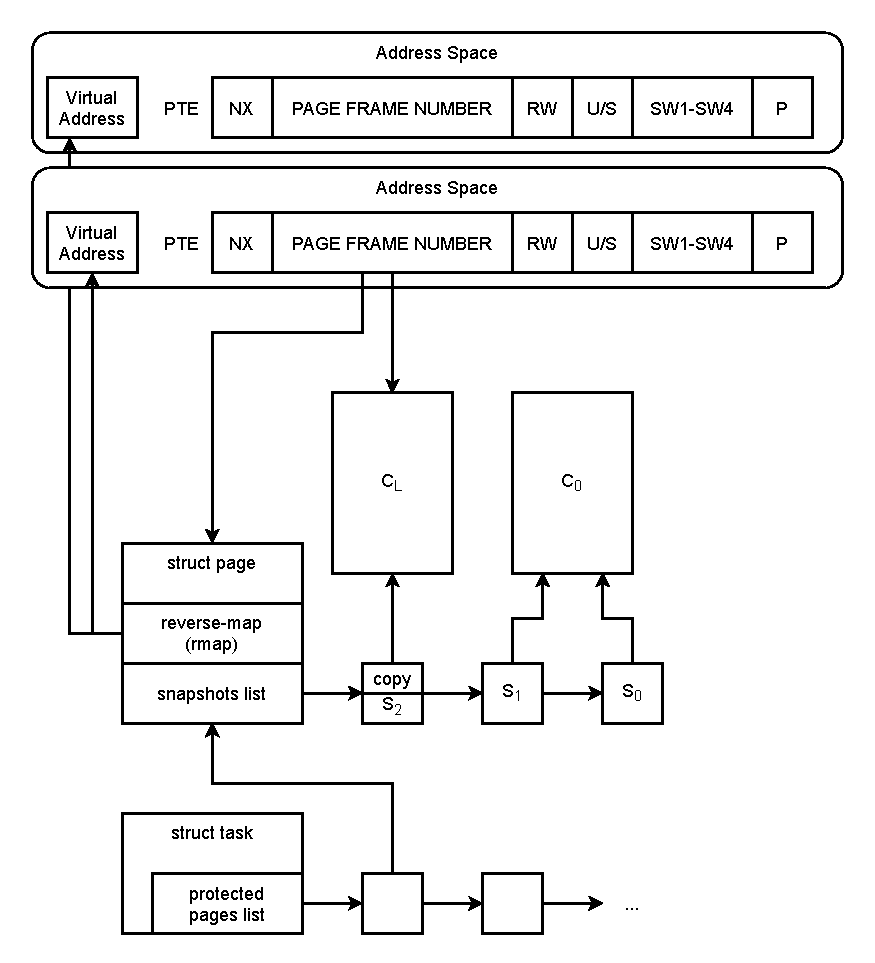
\includegraphics[width=\linewidth]{img/book-keeping.pdf}
  \caption{\sysname{} bookkeeping information. New data structures are in bold. The page frame and marking information are fetched based on the
  page frame number. The marking information is allocated on demand and stored
  in a hashmap to preserve memory.}
  \label{fig:bookkeeping}
\end{figure}

\subsection{Marking and Unmarking}

\begin{figure}[]
  \centering
  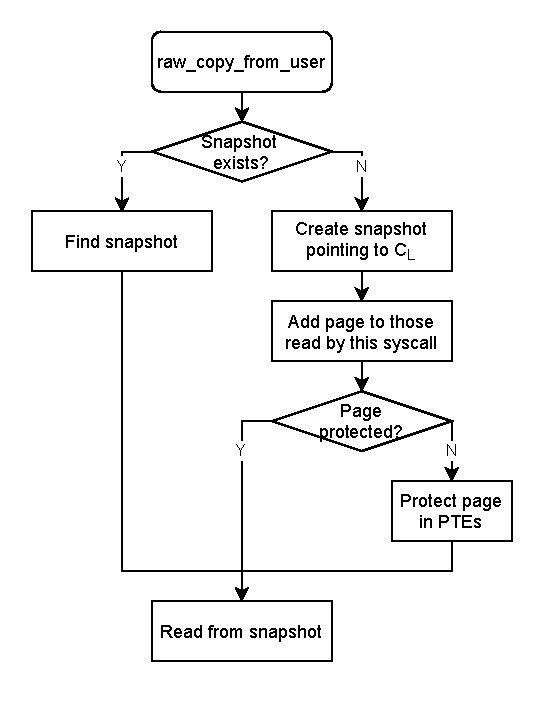
\includegraphics[width = 0.8\linewidth]{img/copy_from_user.pdf}
  \caption{\texttt{copy\_from\_user} page marking. New steps are in bold. Read pages are marked in all VM spaces, as well as their backing files.
}
  \label{fig:copyfromuser}
\end{figure}

\begin{figure}[]
  \centering
  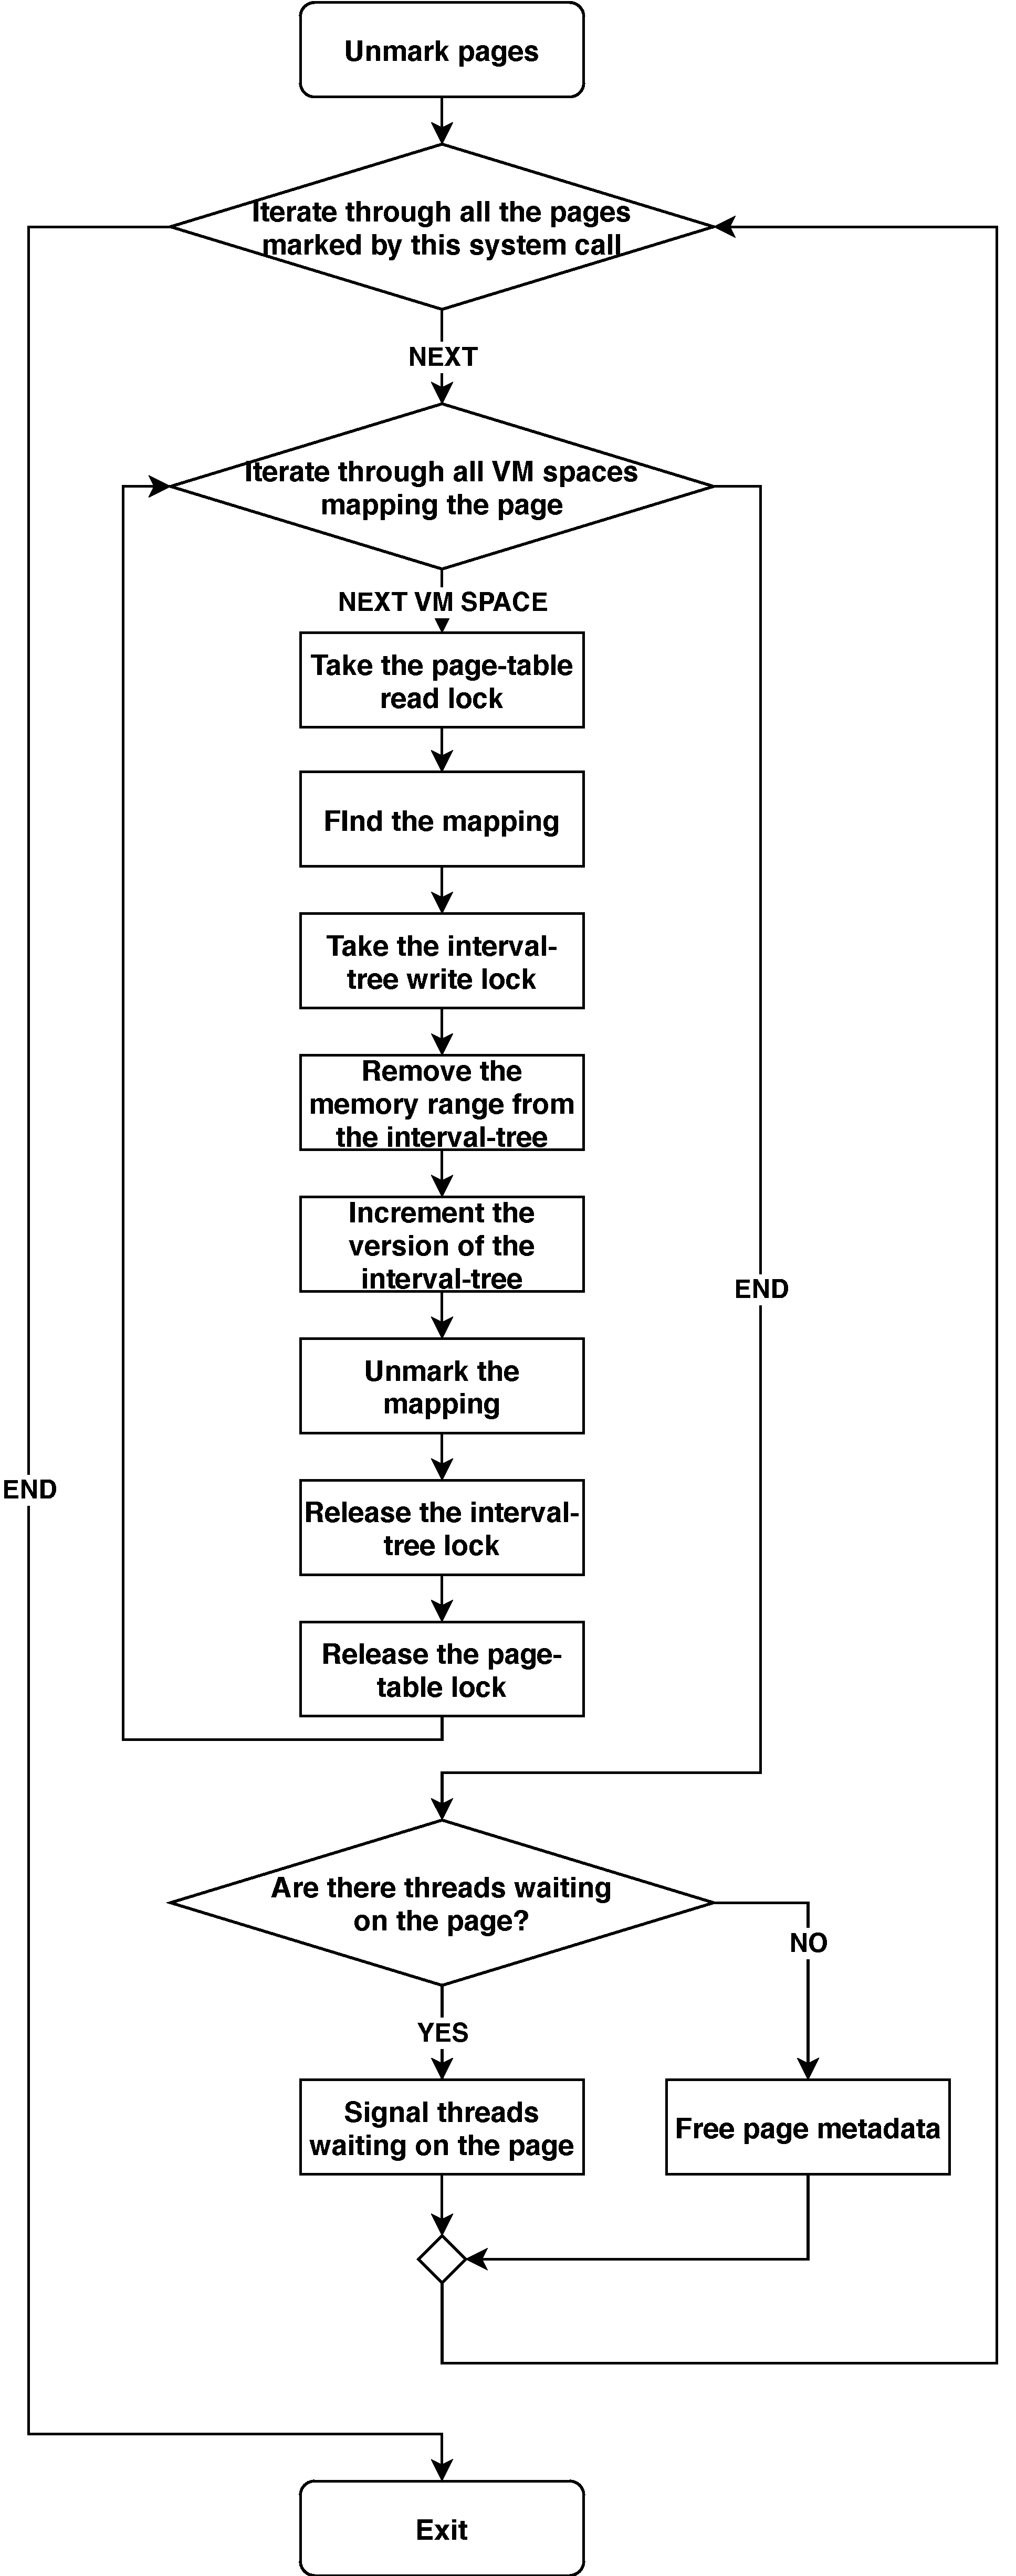
\includegraphics[width = 0.8\linewidth]{img/unmark_pages.pdf}
  \caption{Page unmarking at the end of the system call.
}
  \label{fig:unmarking}
\end{figure}

\sysname{} extends Linux's interface for reading and writing to user-space. The
abstractions \texttt{read\_in} and \texttt{write\_out} introduced in
\autoref{sec:design} are implemented in Linux as \texttt{copy\_from\_user} and
\texttt{copy\_to\_user}. \sysname{} extends \texttt{copy\_to\_user} to mark the pages
before reading the data (\autoref{fig:copyfromuser}).

Marking the page involves taking the appropriate locks, denoting the physical
page frame as marked, and incrementing the number of page owners. \sysname{} then
uses the reverse mapping information to mark the page in all the VM spaces
mapping it.

Unmarking follows a similar procedure (\autoref{fig:unmarking}). The appropriate
locks are taken, and the number of owners is decremented. Only if no owners are
marking the page anymore, it is unmarked in all VM spaces. If threads are
waiting on the page, they are woken up. The last guest to wake up will
deallocate the marking data for the page.


% Deadlock prevention when accessing shared data structures
\subsection{Deadlock Prevention} \label{subsec:deadlockprevention}
%%%%%%%%%%%%%%%%%%%%%%%%%%%%%%%%

Our implementation shares several data structures among multiple threads
(marking information, pages, completions, page-tables, or interval-trees).  To
prevent deadlocks, locks are always taken in increasing order.  The only two
locks taken in two different orders are the \emph{page-table lock} and the
\emph{interval-tree lock}, which protect the marked memory ranges. \sysname{}
features a deadlock prevention mechanism for these locks.


% Locks are taken in opposite orders
In \texttt{copy\_to\_user}~\autoref{fig:copytouser} the interval-tree lock must
be taken first to check which memory ranges are marked. However, when marking a
page the page-table lock needs to be acquired first to locate the page-table
entry mapping the page~\autoref{fig:copyfromuser}. \sysname{} implements the
deadlock resolution mechanism where if the page-fault handler notices that the
interval-tree lock is already taken, it gets released.

% Explain the problematic case when the system call actually waits on a marked
% page. However, if it is waiting it cannot do the exact same thing as the second
% thread and cause a deadlock. There are no waits-for cycle, only chains
The prevention mechanism leads to a way for system calls to write and block
on marked pages. Ultimately, it cannot cause a deadlock because a 
user-thread executing in kernel context would
need to read and write to user-space at the same time. 

The first thread executes \texttt{copy\_to\_user}~\autoref{fig:copytouser} and
attempts a write to page that is not present. This triggers a page-fault which
loads the page. Before the first thread re-executes the write to the page, the
second thread marks it. The first thread cannot abort the write and is forced to
wait. For the second thread to wait for the first, it is necessary for the same
race to happen the second time, with the roles reversed. This is impossible,
as the first thread is waiting due to its attempted write.


\subsection{Loading File-Backed Pages}

% When a marked page is mapped in a different VM space it is marked
% We also need to preallocate memory outside the atomic context
Following our proposed design, file-backed pages need to be marked as
they are loaded to memory. On-demand paging takes place in the page-fault
handler, but invokes the functions of the file-system storing the file. \sysname{}
extends the functionality of \texttt{set\_alloc\_pte} to mark the page. The
needed structures are preallocated and passed into the \emph{atomic context} where 
\texttt{set\_alloc\_pte} is called.

When a marked page is loaded, its data is also added to the interval-tree
storing the marked memory ranges. \sysname{} takes the lock before entering the
atomic context, even though the loaded page may not be marked. The version
number of the interval-tree is incremented after adding the page, informing all
other threads that it has changed.


\subsection{Protecting System Call Arguments from Kernel Writes}
%%%%%%%%%%%%%%%%%%%%%%%%%%%%%%%%%%%%%%%%%%%%%%%%%%%%%%%%%%%%%%%%

\label{subsec:kernelland}
\begin{figure}[]
  \centering
  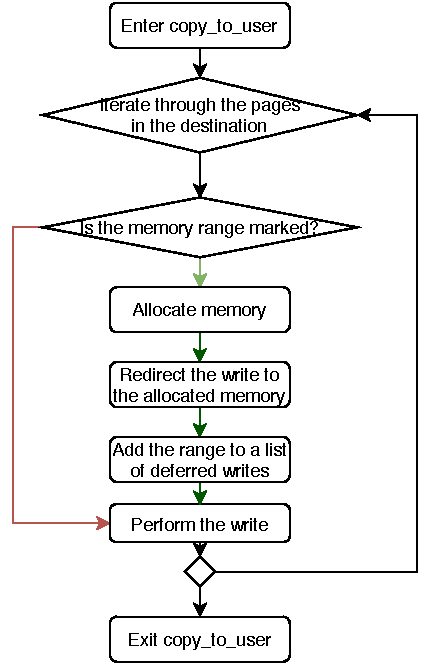
\includegraphics[width = 0.8\linewidth]{img/copy_to_user.pdf}
  \caption{\texttt{copy\_to\_user} write handling. New steps are in bold.
  The write destination is checked for marked ranges. Unmarked ranges are written to, while
  the writes destined for marked ranges are deferred until the end of the system call. Deadlocking
  in the page-fault handler is prevented by releasing the interval-tree lock.
}
  \label{fig:copytouser}
\end{figure}

\begin{figure}[]
  \centering
  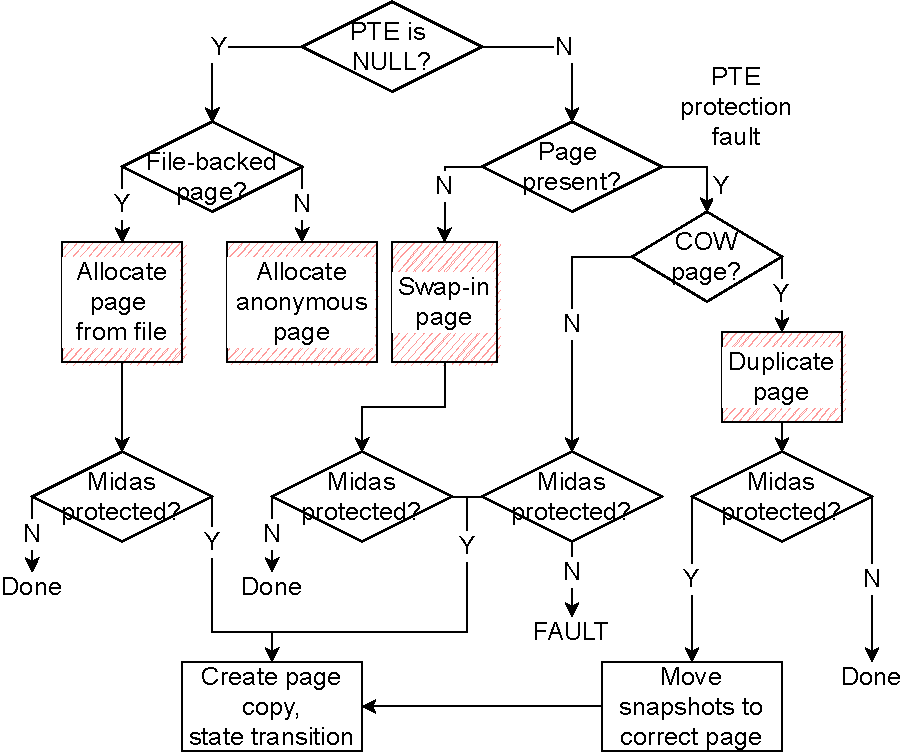
\includegraphics[width = 0.8\linewidth]{img/pagefault.pdf}
  \caption{\sysname's handling of the writes in the page-fault handler. New steps are in bold. Interval-tree lock
  is released at the start of the handler to prevent deadlocks.
}
  \label{fig:pagefault}
\end{figure}

% Before writing to user-space the kernel checks if the page is marked
\sysname{} stores the marked memory ranges for every VM space
(\texttt{mm\_struct}) in an interval tree. Before writing to user-space,
\texttt{copy\_to\_user} (\autoref{fig:copytouser}) acquires the lock for the
marked memory ranges tree and checks for the intersections with the destination
buffer.  Writes to marked pages are stored to freshly allocated memory, along
with the destination address, and written at the end of the call.

% Explain what happens when the target page is not present
Writes to unmarked pages proceed as normal, unless the page is not present. Then
a page-fault exception happens (\autoref{fig:copytouser}). The page-fault
handler takes the page-table lock, loads the page, and restarts the write. If the
page-fault handler detects a potential deadlock, it will release the
interval-tree lock. The page-table read-lock is not exclusive, so it does not need
to be released (\autoref{fig:pagefault}).

% What happens after the fault?
\texttt{copy\_to\_user} will attempt to write to the page after exiting the
page-fault handler. In the case it is indeed marked, it will block and wait for
its unmarking. This is the only case where \sysname{} forces threads to wait in
the middle of a system call and has been explained in
\autoref{subsec:deadlockprevention}. After the write, the thread reacquires the
lock, checks if the interval tree has changed, and restarts the write if so.

% Explain why we restart the write. Doesn't that slow the system down?
The restart of the write is necessary because any change to the interval-tree
invalidates the iterator. \sysname{} is optimized for the case of rare markings,
making \texttt{copy\_to\_user} calls that do not encounter marked pages fast as
only a single, large write occurs. The alternative is to check and write to every
page individually. Such implementation does not need to restart the write but
incurs the overhead of individually writing to pages.


%%%%%%%%%%%%%%%%%%%%
\section{Evaluation} \label{sec:evaluation}
%%%%%%%%%%%%%%%%%%%%

% We want to test TikTok on programs with many threads and/or processes, and on
% programs that use many system calls. That is where we expect to lose performance

To fully evaluate the impact of our memory marking system, we need to carefully
consider a variety of different usage scenarios both in user-centric (desktop)
environments as well as server environments. We build on the large body of
existing systems benchmarks to demonstrate performance impact of our system.

\sysname{} has most impact when marking and unmarking pages during
system calls. This overhead is proportional to the number of VM spaces
(processes) that have the pages mapped. Benchmarks must measure the \sysname{}
overhead for the multithreaded and multiprocessed workloads, as well as the
workloads with many marking system calls.

% Based on the previous section we have picked these benchmarks
We evaluate \sysname{} using two different benchmark suites: the NAS Parallel
Benchmark (NPB)~\cite{npb} and the Phoronix Test Suite (PTS)~\cite{pts}. NPB
tests \sysname{} on multithreaded or multiprocessed CPU-bound workloads. NPB is
a suitable benchmark to measure a drop of performance due to multithreading and
multiprocessing. PTS evaluates \sysname{} on several real-world applications.
They complement NPB in that they consist of system call heavy applications, with
varying degrees of parallelism. In this evaluation we do not include results of
SPEC CPU2006 or SPEC CPU2017 as that benchmark is heavily CPU bound and
optimized to have minimal interaction with the operating system, i.e., the
number of system calls is extremely low resulting in negligible overhead.

% My office desktop machine and the kernel I cloned a year ago
All benchmarks have been performed on Ubuntu Server 18.04 LTS (Linux 5.4.0-rc3)
with Intel i7-9700 and 16 GB of RAM.
%
We compare three main \sysname{} configurations:
\begin{LaTeXdescription}
  \item[\sysname{} On] full protection of system calls,
  \item[\sysname{} Partial] whitelists the \texttt{write}
system call and variants (\texttt{pwrite}, \texttt{pwrite64}, \texttt{pwritev}), and
  \item[\sysname{} Off] is the Linux kernel compiled without \sysname{}. 
\end{LaTeXdescription}


\subsection{NAS Parallel Benchmark} \label{subsec:npb}
%%%%%%%%%%%%%%%%%%%%%%%%%%%%%%%%%%%

% A bit more about the benchmark
\emph{NAS Parallel Benchmarks (NPB)}~\cite{npb} is a benchmark introduced by
NASA. It consists of several parallel programs using different communication
patterns. \sysname{} introduces additional synchronization points between
threads, so it should affect multi-threaded programs more than single-threaded
ones. NPB is available for multiple technology stacks for parallel programming.
\sysname{} was evaluated on \emph{OpenMP}~\cite{dagum1998openmp} and
\emph{MPI}~\cite{snir1998mpi} versions of the benchmark with workloads of class
A.

\begin{figure}[]
  \centering
  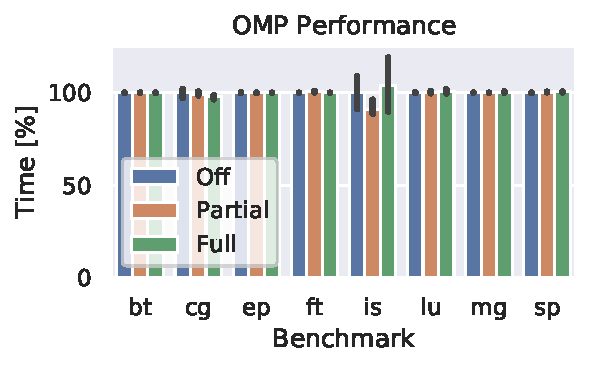
\includegraphics[width=\linewidth]{img/omp_graph.pdf}
  \caption{\sysname{} evaluated on NPB with OMP.
}
  \label{fig:npbomp}
\end{figure}

\begin{figure}[]
  \centering
  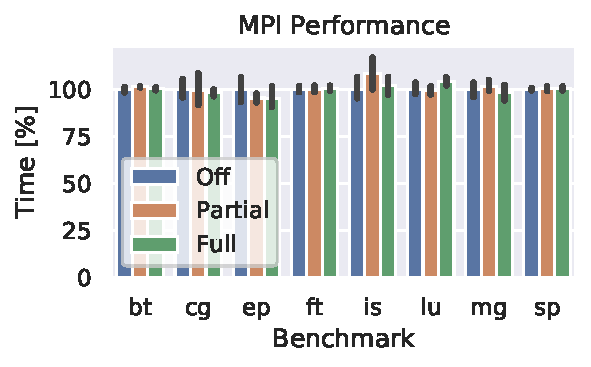
\includegraphics[width=\linewidth]{img/mpi_graph.pdf}
  \caption{\sysname{} evaluated on NPB with MPI.}
  \label{fig:npbmpi}
\end{figure}

% Two variants that test either threads or processes

OpenMP~\cite{dagum1998openmp} is a compiler extension that splits the execution
to multiple threads. All threads still use the same VM space, keeping the
overhead minimal. \sysname{} was evaluated with 8 threads.

MPI~\cite{snir1998mpi} implements parallel execution by launching multiple
processes which communicate by message-passing. Due to the limitations of some
benchmarks, \sysname{} was evaluated with 16 processes.

% We interpret the results
The benchmarks have been run with \sysname{} protecting almost all calls, with
\texttt{write} variants disabled and without \sysname{} at all
(\autoref{fig:npbomp} and \autoref{fig:npbmpi}). Both benchmarks show no
significant difference between different setups. MPI has wider standard-error
margins, probably introduced by the heavier startup and communication. Shorter
benchmarks magnify relative differences (explaining the artifacts for
\texttt{is} and \texttt{ep}). \sysname{} does not incur a noticeable performance
penalty for CPU-bound workloads, even when they involve multiple
threads/processes.


\subsection{Phoronix Test Suite} \label{subsec:phoronix}
%%%%%%%%%%%%%%%%%%%%%%%%%%%%%%%%

\begin{figure*}[]
  \centering
  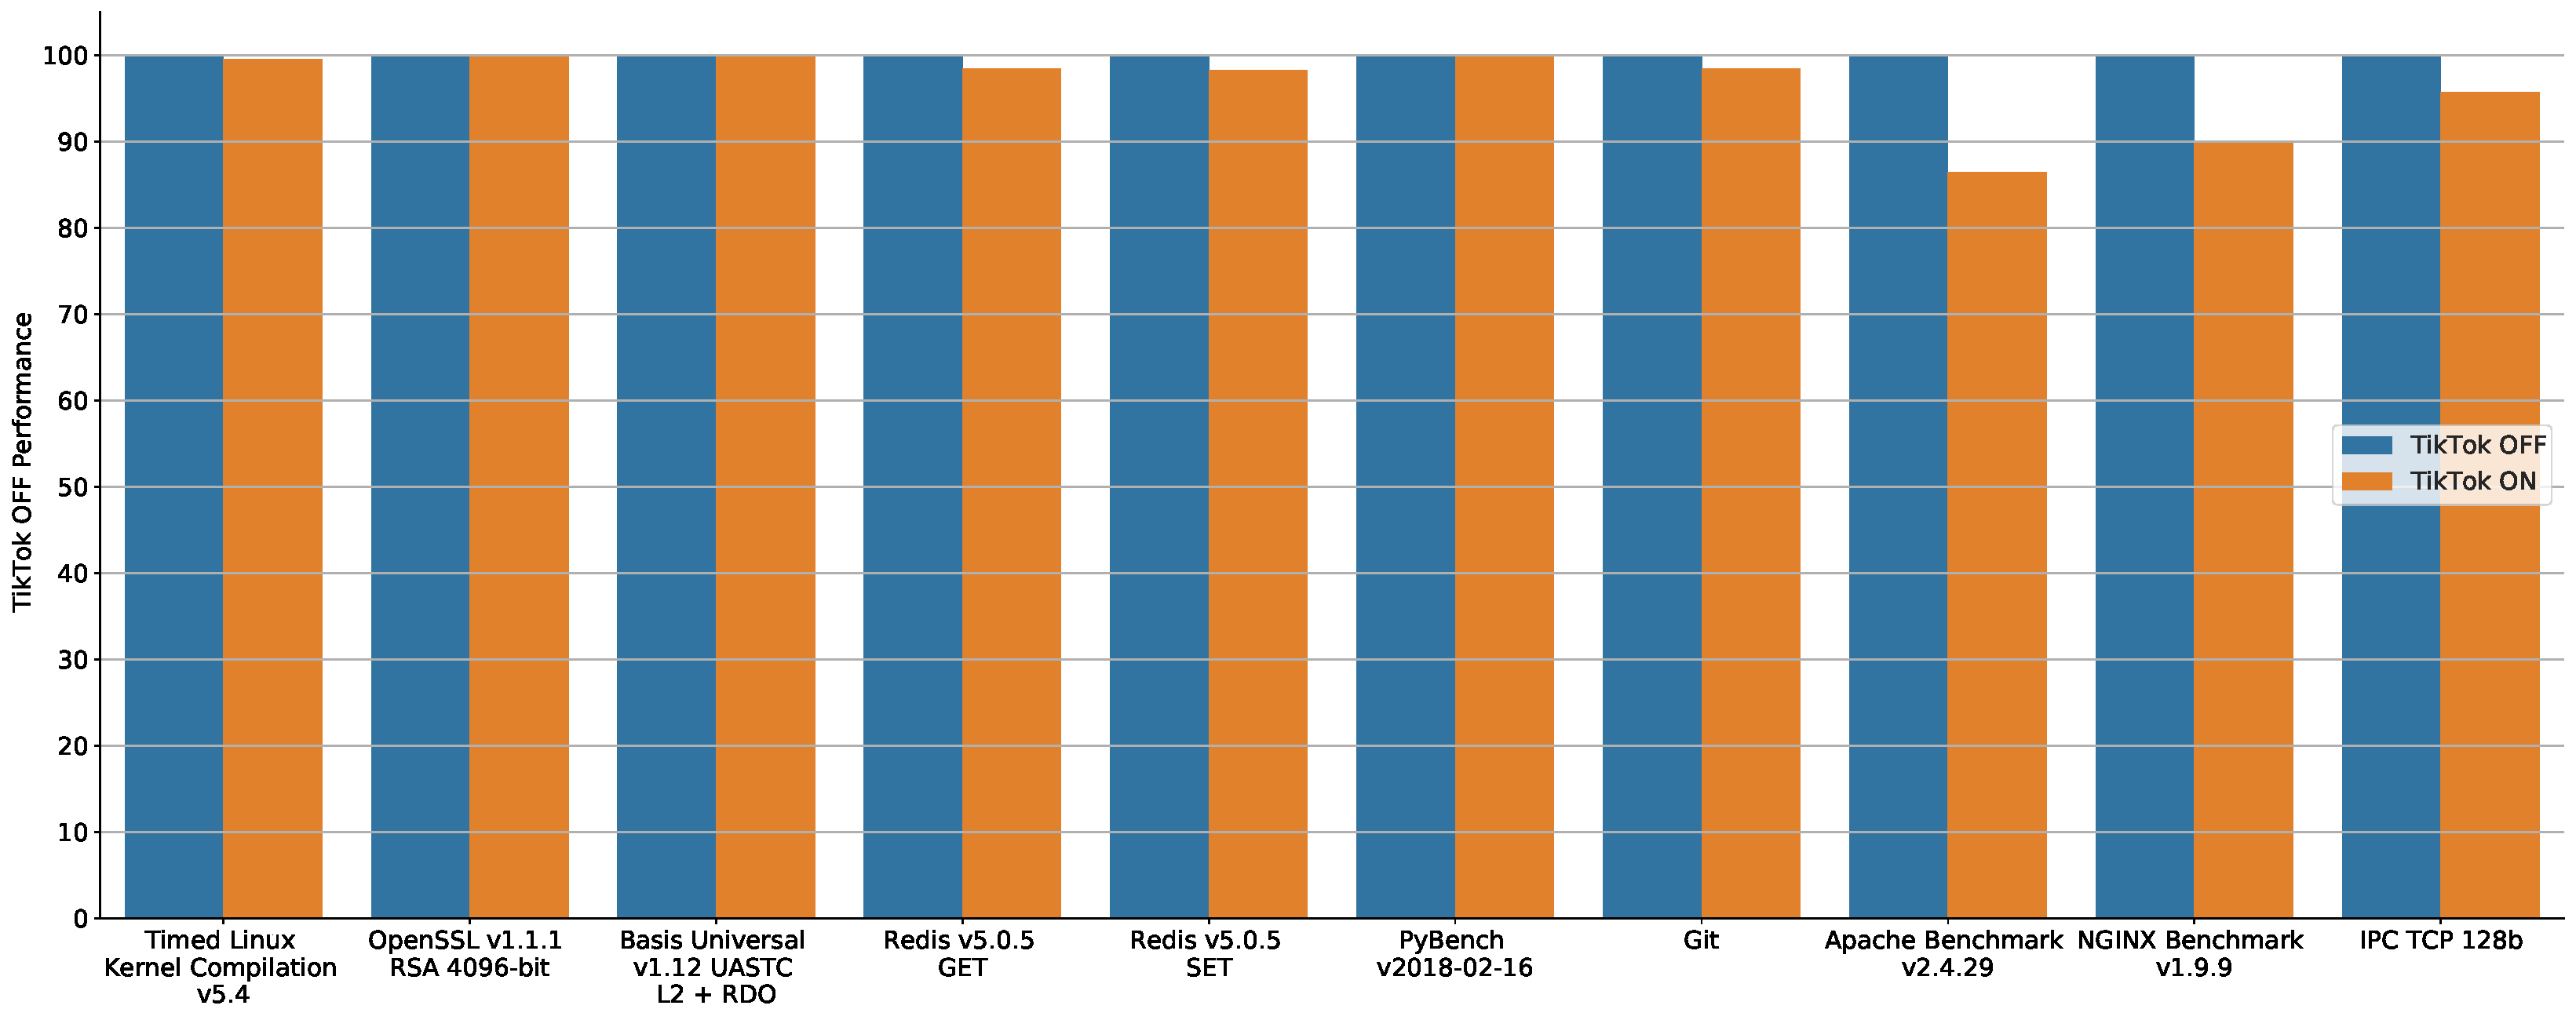
\includegraphics[width=\linewidth]{img/eval.pdf}
  \caption{\sysname{} evaluation on Phoronix Test Suite.
}
  \label{fig:phoronix}
\end{figure*}

% Explain why we used it in a bit more detail
\emph{Phoronix Test Suites (PTS)}~\cite{pts} evaluates systems on real-world
software. PTS tested \sysname{} on a range of programs complementing NPB:
from single-threaded, CPU-bound applications (OpenSSL) to multi-threaded,
multi-processed, programs with frequent system calls (Apache).

% Explain how to read the graphs
\autoref{fig:phoronix} shows the results of the Phoronix benchmark. All results
have been normalized with respect to '\sysname{} Off'. Benchmarks marked
with an asterisk (*) measure execution time (lower is better), while others
measure performance (higher is better).

% Benchmarks which show no performance loss
Linux compilation, OpenSSL, Redis, Git and PyBench do not show a noticable
degradation in performance. These programs do not feature a lot of inter-process
communication. Even the parallelized benchmarks such as Linux kernel compilation
generate independent, non-communicating processes.

% Three benchmarks which slow down
However, the two web servers (Apache and NginX) show a significant drop in
performance (16.87\% for Apache and 16.38\% for NginX) with \sysname{}
protecting all calls. Whitelisting write calls improves the situation slightly
(15.64\% for Apache and 13.41\% for NginX). \sysname{} affects parallel and
applications with numerous system calls the most because of the marking
overhead. The impact of whitelisting write calls is small due to the low
frequency of calls.

The IPC TCP benchmark consists of two system calls that transfer data between
two threads. Compared to other benchmarks, IPC benchmark has fewer threads than
web-servers, but also executes a significant number of system calls. This places
it in-between two groups with respect to the performance penalty.

\begin{figure}[]
  \centering
  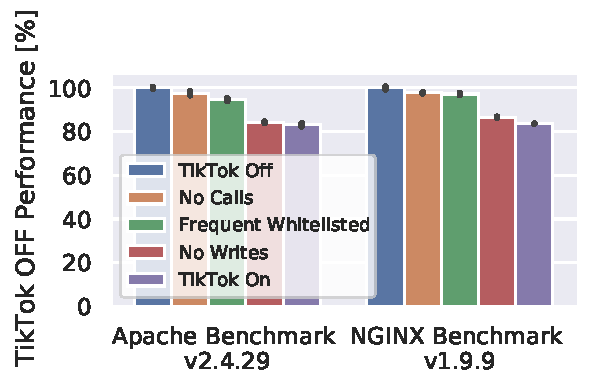
\includegraphics[width=\linewidth]{img/freq_removed.pdf}
  \caption{Detailed comparison of Apache and NginX performance.}
  \label{fig:phoronix-apache-nginx}
\end{figure}


% More detailed results
\subsection{Apache and NginX Overhead breakdown}
%%%%%%%%%%%%%%%%%%%%%%%%%%%%%%%%%%%%%%%%%%%%%%%%

We evaluated the Apache and NginX benchmarks under two additional \sysname{}
configurations to more accurately assess the effect of system calls on
performance (\autoref{fig:phoronix-apache-nginx}):

\begin{LaTeXdescription}
  \item[Frequent system calls whitelisted] whitelists the most frequent calls
  executed in the benchmarks (\texttt{epoll\_ctl}, \texttt{close},
  \texttt{read}, \texttt{fcntl}, \texttt{connect}, \texttt{recvfrom},
  \texttt{epoll\_wait}, \texttt{accept4}, \texttt{openat}, \texttt{socket},
  \texttt{shutdown}, \texttt{fstat}, \texttt{sendfile}, \texttt{stat},
  \texttt{mmap}, \texttt{munmap}, \texttt{getsockname}, \texttt{times}), as well
  as \texttt{write} and its variants. The code of standard system calls has been
  checked for double-fetches in previous work~\cite{wang2017double,
  xu2018precise}. \texttt{mmap} and \texttt{munmap} do not read memory and mark
  pages. Therefore, they are safe to whitelist.


  \item[All system calls whitelisted] does not protect any system calls.
\end{LaTeXdescription}

Whitelisting frequent system calls leads to a smaller overhead (Apache -- 5.34\% and
NginX -- 2.77\%). The performance is almost equal to not protecting any
system calls at all (Apache -- 2.46\% and NginX -- 2.25\%). Some overhead
remains even when \sysname is not protecting any calls because
\texttt{copy\_to\_user} protection is still active.

\begin{table*}[]
  \label{perftable}
  \centering
  \begin{tabular}{|l|l|l|l|l|}
  \hline
                                     & Apache (\sysname{} Off) & Apache (\sysname{} - No writes) & IPC (\sysname{} Off) & IPC (\sysname{} - No writes)\\ \hline
  Marking pages read-only            & 0\%    & 5.22\%          & 0\% & 0\%         \\ \hline
  Unmarking pages                    & 0\%    & 4.67\%          & 0\% & 0.94\%      \\ \hline
  Flushing Individual TLB Ranges     & 1.50\% & 6.96\%          & 0\% & 0\%         \\ \hline
  Shared Write Buffers Protection    & 0\%    & 0.05\%          & 0\% & 1.72\%      \\ \hline
  \texttt{copy\_to\_user} Protection & 0\%    & 1.93\%          & 0\% & 1.28\%      \\ \hline
  Measured Overhead                  & 0\%    & 18.56\%         & 0\% & 4.72\%      \\ \hline
  \end{tabular}
  \caption{Perf Analysis of the Benchmarks. The percentages are normalized to \sysname{} Off execution times.}
\end{table*}

% I have picked two benchmarks with different behaviors and a high TikTok overhead
% They were tested on the TikTok configuration that should make the differences evident
To contrast the overhead between two different workloads, we traced Apache and IPC
with \texttt{perf}. The traces serve as ground truth
(\sysname{} Off) and \sysname{} with writes whitelisted. Here, the IPC benchmark
does not incur any marking overhead, while Apache still marks pages.

% How to read the table. TLB data is already included in marking and unmarking
\autoref{perftable} shows how much time the programs spend in
\sysname{} functions. We measure percentages of individual segments with
\texttt{perf}, while calculating the total overhead from the results of the
benchmarks. While the TLB is flushed both during the marking and unmarking of
pages, but is included in the table as an important performance parameter.

% Explain the differences
The comparison of the Apache and IPC runs shows two very different marking
profiles. Apache spends a considerable amount of time marking and unmarking
pages, while IPC does not mark pages at all. This is a consequence of the
different system calls used by these applications. IPC uses only \texttt{read}
and \texttt{write} calls which do not mark arguments, while Apache also invokes
marking system calls (\texttt{accept}, \texttt{getsockname}).

% TLB flushes slow down the programs
Apache waits most of the time for the TLB signaling functions to execute.
\texttt{flush\_tlb\_mm\_range} amounts for 2.51\% (marking) and 2.16\%
(unmarking) of the total time spent executing the benchmark. Frequent TLB
flushes are expensive because the CPU needs to make sure that all the cores have
processed the signal before continuing. Flushed pages will be accessed right
afterward, leading to a TLB miss. This further inflates the overhead.

% IPC is slowed down due to the passive protection
IPC benchmark executes only \texttt{write} and \texttt{read} calls. It does not
incur any overhead on TLB flushes because none of these calls mark pages.
However, \texttt{copy\_to\_user} checks are still active, causing a noticeable
locking overhead.


%%%%%%%%%%%%%%%%%%%%%%
\section{Related Work} \label{sec:relatedwork}
%%%%%%%%%%%%%%%%%%%%%%

% Static and dynamic solutions for DFs
The literature related to double-fetches can be broadly divided into two groups.
Static solutions are in the first group. These systems use techniques such as
source or binary analysis to detect double-fetch bugs. The second group of
systems uses run-time information to detect and (rarely) prevent double-fetches.

The most inspiring work related to \sysname{} is the paper by
Watson~\cite{watson2007exploiting}, criticizing the security of system call
wrappers.


% Go over Watson's paper. Tell everyone he found lots of problems and that we
% fixed all of them
\subsection{Watson's Critique of System Call Wrappers} \label{subsec:watson}
%%%%%%%%%%%%%%%%%%%%%%%%%%%%%%%%%%%%%%%%%%%%%%%%%%%%%%

Watson's paper~\cite{watson2007exploiting} scrutinized the security of many
system call wrappers. Not only did he discover that all existing system call
wrappers were fundamentally insecure, Watson also described the different types
of TOCTTOU bugs that compromised them and discussed potential fixes. In a short
paragraph, he mentions that Pawel Dawidek, the creator of
CerbNG~\cite{zak_frasunek_dawidek}, has experimented with marking arguments
read-only. CerbNG was an early system call filtering system for BSD that used
copy-on-read-and-write to a new memory page.  Our very first design sketch
followed a similar idea but we quickly discovered the potential drawbacks that
remained.

Afterward, Watson briefly discusses problems such memory marking systems
must solve: 
\begin{itemize}
    \item unnecessary page-faults,
    \item bypassing memory marking using IO system calls,
    \item mapping shared memory with different permissions, and
    \item handling system calls that both read and write to the same memory.
\end{itemize}

According to Watson, no memory-marking system (including CerbNG) addressed all
of these pervasive problems. \sysname{} does exactly that and even includes
protection against new attacks that Watson was not aware of. Unnecessary
page-faults are rare and they are used to make the offending threads wait for
unmarking. After the page has been unmarked, the write proceeds without any
consequences. Write system calls do not proceed until there are no marked pages
of the file. Pages are marked when they are mapped and only if needed.
\sysname{} postpones all writes to marked pages coming from the kernel while
allowing the system calls to execute correctly.


% Static analysis---Good at finding bugs, you do not need to run the code.
% It does not find DFs in binaries and it does not fix bugs
\subsection{Static Analysis Work} \label{subsec:dfstatic}
%%%%%%%%%%%%%%%%%%%%%%%%%%%%%%%%%

Static analysis techniques analyze the source code to find double-fetch bugs.
Wang et al.~\cite{wang2017double} used pattern matching to find potential
double-fetches. They implemented a tool that patches certain double-fetches
automatically. However, their method in the general case produces false
positives that must be manually inspected. Xu et al.~\cite{xu2018precise}
improved on this work by proposing \emph{Deadline}. Deadline does not use the
pattern analysis on the source files to detect double-fetches, but a compiler's
intermediate representation and constraint solving to reduce false positives.

Static analysis techniques such as these have the benefit of discovering
bugs in the code that cannot be run (e.g., mitigating the need for specific
hardware to test a particular driver). However, they are meant for bug
detection, not mitigation. Even though the tools can discover some bugs
automatically, this is not always possible. System call wrappers have, by
design, an inherent TOCTTOU bug.

Double-fetches introduced by the compiler are another challenge. While the
source code and even the intermediate representation may be bug free, the
compiler can introduce such ``invisible'' double-fetches when allocating
registers to variables. \sysname{} protects the system against all kinds of
double fetches.


% Dynamic analysis---You are limited to the code you can run. You can find
% DFs introduced by compilers. Schwartz and al. have an amazing idea to mitigate
% DFs using TSX. Unfortunately, TSX limits the protected code quite a bit
\subsection{Dynamic Analysis Work} \label{subsec:dfdynamic}
%%%%%%%%%%%%%%%%%%%%%%%%%%%%%%%%%%

Google Project Zero's Bochspwn~\cite{jurczyk2013bochspwn} uses an emulator to
detect double-fetches. It found a large number of bugs in the Windows kernel.
Bochspwn works on binaries (i.e., it needs no source code access) and
detects bugs introduced by compilers. DFTracker~\cite{wang2019dftracker} is
another dynamic analysis technique, with a lower overhead, that relies on
taint tracking. However, these dynamic techniques are limited in their detection
of double-fetches. First, similar to work presented in \autoref{subsec:dfstatic},
developers need to manually fix all discovered bugs. Second, in contrast to
static techniques, with dynamic analysis the double-fetch must also be executed
by some concrete code and input, limiting this technique to the core kernel
and to the drivers with the available hardware.

A big leap in dynamic analysis techniques has been presented by Schwartz et
al.~\cite{schwarz2018automated}. The first part of the paper introduces DECAF,
a framework that uses side-channel attacks to create a fuzzing oracle for
double-fetch bugs. While Bochspwn relies on emulation, slowing the execution
significantly, DECAF runs natively. It also eliminates false positives by
automatically exploiting found bugs.

Schwartz et al. then discuss DropIt, a real-time mitigation technique for double
fetches. DropIt uses Intel's \emph{Transactional Synchronization Extensions}
(TSX)~\cite{intel64and} in a creative way to prevent double-fetch bugs. By
encapsulating the code in a TSX transaction, writes from other threads will
result in the transaction being aborted. However, the code executing inside a
TSX transaction is severely limited. All reads must fit in the L3 cache, and all
writes in L1. Some instructions are also forbidden. \sysname{} faces none of those
limitations. It works on non-Intel processors and relies on page tables for
protection, a technique that has been present for several decades.


% We can port TikTok to other systems and arches, use it to protect filters,
% maybe even optimize it a bit
%%%%%%%%%%%%%%%%%%%%
\section{Discussion} \label{sec:discussion}
%%%%%%%%%%%%%%%%%%%%

\sysname{} can be ported to any kernel that accesses user-space memory through a
well-defined interface, and any computer architecture that features page-tables.
Android devices frequently have binary-only drivers and porting \sysname{} to
ARM would provide additional safety guarantees to the Android ecosystem.

Current system call filters~\cite{landlock,krsi} prohibit TOCTTOU races by
implementing filters as Linux Security Module (LSM)~\cite{morris2002linux}
hooks. For the filters to work, LSM hooks need to be present in drivers. Even
then, the undesired behavior may manifest before a hook is encountered.
Integration of \sysname{} with an existing system call wrapper would solve these
TOCTTOU races.  SecComp~\cite{seccomp} and eBPF~\cite{ebpf} are the obvious
candidates that would benefit from such an extension. \sysname{} performance
could be improved by marking only the pages that are read by the filter in
the system call wrapper.

The performance overhead of \sysname{} for multithreaded, system call heavy
applications is low but not negligible due to the marking overhead. A
possibility of batching TLB flushes for multiple pages should be explored as a
possible optimization.


%%%%%%%%%%%%%%%%%%%%
\section{Conclusion}
%%%%%%%%%%%%%%%%%%%%

% Abstract Ctrl+C Ctrl+V
\sysname{} mitigates double-fetch bugs in system calls by using page-tables. It
works both on the core kernel, and drivers, even when their source code is not
available. It can be ported to any architecture that uses page-tables, and any
kernel that has a well-defined interface to access user-space memory. 

Our prototype implementation of \sysname{} for x86-64 protects modern systems
(e.g., Ubuntu Server 18.04 LTS) with complex programs running (\texttt{systemd},
\texttt{gcc}, \texttt{Apache}). When protecting rare system calls our mitigation
incurs a negligible overhead of \roughevaloverheadbetter{}, which raises to a
low overhead of \roughevaloverheadbad{} when protecting almost all calls in
multithreaded, system call intensive programs. CPU-bound programs do not have a
significant overhead, even if they use multiple threads.


%-------------------------------------------------------------------------------
%\section*{Acknowledgments}
%-------------------------------------------------------------------------------

%-------------------------------------------------------------------------------
\section*{Availability}
%-------------------------------------------------------------------------------

The source code of TikTok is available at LINK. It has been released under the
GNU Public Licence.

%-------------------------------------------------------------------------------
\bibliographystyle{plain}
\bibliography{TikTok}

%%%%%%%%%%%%%%%%%%%%%%%%%%%%%%%%%%%%%%%%%%%%%%%%%%%%%%%%%%%%%%%%%%%%%%%%%%%%%%%%
\end{document}
%%%%%%%%%%%%%%%%%%%%%%%%%%%%%%%%%%%%%%%%%%%%%%%%%%%%%%%%%%%%%%%%%%%%%%%%%%%%%%%%

%%  LocalWords:  endnotes includegraphics fread ptr nobj noindent
%%  LocalWords:  pdflatex acks
